\begin{appendices}
	\chapter{Mitochondrial density is regulated by UNC-16/JIP3 and UNC-76/FEZ1}
	
	
	\large \textbf{UNC-16/JIP3 and UNC-76/FEZ1 limit the density of mitochondria in \textit{C. elegans} neurons by maintaining the balance of anterograde and retrograde mitochondrial transport}
	
	\small
	Guruprasada Reddy Sure, Anusheela Chatterjee, Nikhil Mishra, \textbf{Vidur Sabharwal}, Swathi Devireddy, Anjali Awasthi, Swetha Mohan, Sandhya P Koushika
	
	Publication date : 12 June 2018
	Journal : Scientific Reports
	Volume : 8
	Issue : 1
	doi : \href{https://doi.org/10.1038/s41598-018-27211-9}{10.1038/s41598-018-27211-9}
	
	\normalsize
	My contributions to the following study include  quantification of the molecular motor subunits \textit{unc-116}, \textit{klc-2}, and \textit{dhc-1} RNA levels to assess if the observed change in mitochondrial distribution in \textit{unc-76} and \textit{unc-16} mutants was due to altered motor RNA levels. While the motor RNA levels were unchanged, we did observe an increase in kinesin-1 subunits UNC-116 and KLC-2 protein levels. I further reanalyzed data for multiple figures and re-plotted them for the final representation. Data from this paper are used under the Creative Commons CC-BY license used by Springer Nature Scientific Reports.
	
	\begin{figure}[H]
		\centering
		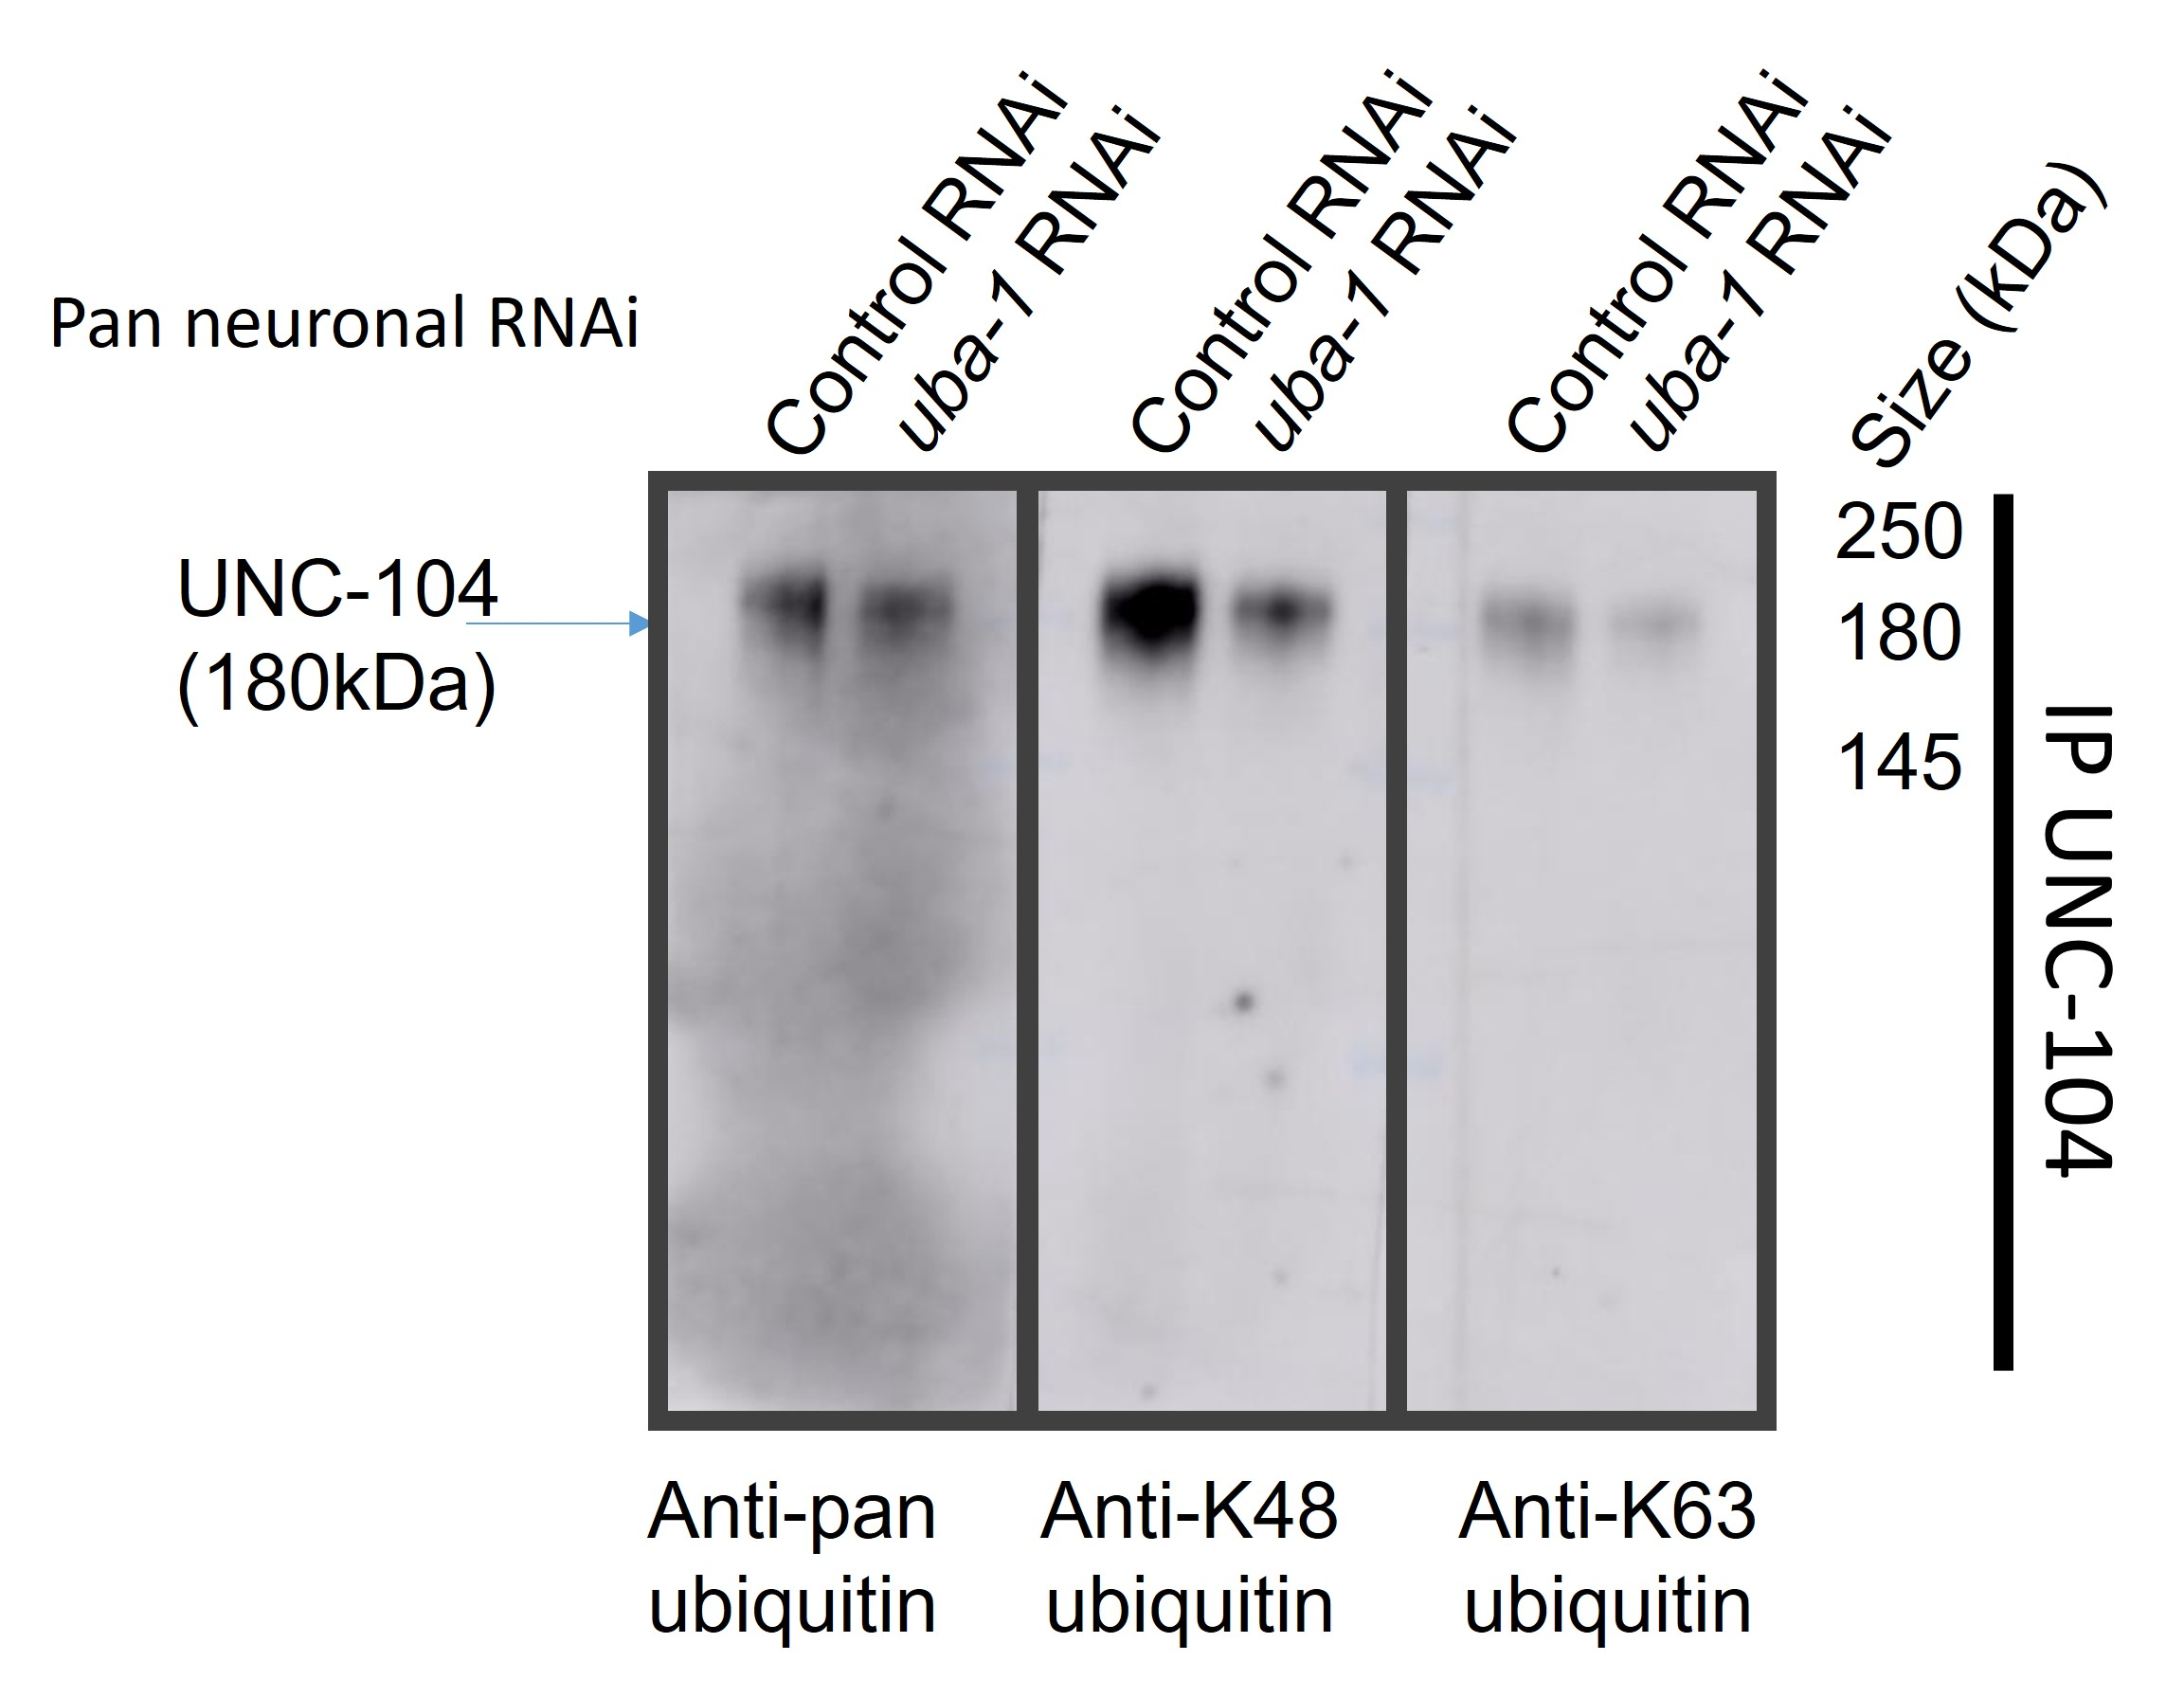
\includegraphics[width=0.8\linewidth]{figs/example}
		\caption[RNA levels of molecular motor subunits \textit{unc-116}, \textit{klc-2}, and \textit{dhc-1} in \textit{unc-16} and \textit{unc-76} mutants.]{\textbf{RNA levels of molecular motor subunits \textit{unc-116}, \textit{klc-2}, and \textit{dhc-1} in \textit{unc-16} and \textit{unc-76} mutants.}} \raggedright \small Fold change in RNA levels of molecular motor subunits \textit{unc-116}, \textit{klc-2}, and \textit{dhc-1} in wild type, \textit{unc-16}, and \textit{unc-76} mutants assessed using $\Delta \Delta$Ct method. Filled circles represent individual data points with the thick dotted line representing the median and thin dotted lines representing the 25\textsuperscript{th} and 75\textsuperscript{th} percentiles. Kruskal Wallis with Dunn's test was used for statistics. ns - non significant. All N=4.
		\label{fig:AnusheelaqPCR}
	\end{figure}
	
	
	\newcolumntype{L}{>{\RaggedRight\hangafter=1\hangindent=1.5em}X}
	\begin{table}[H]\centering
		\caption{Strain list used in this study}\label{tab:StrainlisB}
		\scriptsize
		\begin{tabularx}{1\textwidth}{@{} l l L l @{}}\toprule
			S. No. &Strain name &Genotype &Reference \\\midrule
			1 &N2 &wild type &\cite{brenner1974} \\
			2 & &\textit{unc-16(e109)} &\cite{iwasaki1995} \\
			3 &TT130 &\textit{unc-16(tb109)} abbreviated as unc-16(lf) &\cite{choudhary2017} \\
			4 & &\textit{unc-76(n2398)} &\cite{bloom1997} \\
			5 & &\textit{unc-76(rh116)} &\cite{bloom1997} \\
			\bottomrule
		\end{tabularx}
	\end{table}
	
	\begin{table}[H]\centering
		\caption{Primer list used in this study}\label{tab:PrimerlistB}
		\scriptsize
		\begin{tabularx}{1\textwidth}{@{} l l l l @{}}\toprule
			S. No. &Primer TT no. &Primer name &Primer sequence \\\midrule
			1 &TTpr36 &UNC-116 qPCR FP &CGGAAAAACACATACAATGGAGGGAGTAATCG \\
			2 &TTpr37 &UNC-116 qPCR RP &CTCGGGGTCTAATAAATCTCGAATCTTCTCG \\
			3 &TTpr38 &KLC-2 qPCR FP &CGCCAAAGTTGATAGTCCAACCGTC \\
			4 &TTpr39 &KLC-2 qPCR RP &CTGTTTCTTTGCTCTCAAGGCGACATC \\
			5 &TTpr40 &qRT act-1 FP2 &AGACAATGGATCCGGAATGTGCAAGG \\
			6 &TTpr41 &qRT act-1 RP2 &GGTACTTGAGGGTAAGGATACCTCTCTTGG \\
			7 &TTpr46 &DHC-1 cDNA FP &CTCTCGGACAAGTTTGGGATGC \\
			8 &TTpr47 &DHC-1 cDNA FP &CATCCCATCCTTTGATCAAACGTGTC \\
			\bottomrule
		\end{tabularx}
	\end{table}
	
\end{appendices}
